\documentclass[a4paper,11pt]{article}
\usepackage{amsmath,amsthm,amsfonts,amssymb,amscd,amstext,vmargin,graphics,graphicx,tabularx,multicol} 
\usepackage[francais]{babel}
\usepackage[utf8]{inputenc}  
\usepackage[T1]{fontenc} 
\usepackage{pstricks-add,tikz,tkz-tab,variations}
\usepackage[autolanguage,np]{numprint} 
\usepackage{calc}

\setmarginsrb{1.5cm}{0.5cm}{1cm}{0.5cm}{0cm}{0cm}{0cm}{0cm} %Gauche, haut, droite, haut
\newcounter{numexo}
\newcommand{\exo}[1]{\stepcounter{numexo}\noindent{\bf Exercice~\thenumexo} : }
\reversemarginpar

\newcommand{\bmul}[1]{\begin{multicols}{#1}}
\newcommand{\emul}{\end{multicols}}

\newcounter{enumtabi}
\newcounter{enumtaba}
\newcommand{\q}{\stepcounter{enumtabi} \theenumtabi.  }
\newcommand{\qa}{\stepcounter{enumtaba} (\alph{enumtaba}) }
\newcommand{\initq}{\setcounter{enumtabi}{0}}
\newcommand{\initqa}{\setcounter{enumtaba}{0}}

\newcommand{\be}{\begin{enumerate}}
\newcommand{\ee}{\end{enumerate}}
\newcommand{\bi}{\begin{itemize}}
\newcommand{\ei}{\end{itemize}}
\newcommand{\bp}{\begin{pspicture*}}
\newcommand{\ep}{\end{pspicture*}}
\newcommand{\bt}{\begin{tabular}}
\newcommand{\et}{\end{tabular}}
\renewcommand{\tabularxcolumn}[1]{>{\centering}m{#1}} %(colonne m{} centrée, au lieu de p par défault) 
\newcommand{\tnl}{\tabularnewline}

\newcommand{\trait}{\noindent \rule{\linewidth}{0.2mm}}
\newcommand{\hs}[1]{\hspace{#1}}
\newcommand{\vs}[1]{\vspace{#1}}

\newcommand{\N}{\mathbb{N}}
\newcommand{\Z}{\mathbb{Z}}
\newcommand{\R}{\mathbb{R}}
\newcommand{\C}{\mathbb{C}}
\newcommand{\Dcal}{\mathcal{D}}
\newcommand{\Ccal}{\mathcal{C}}
\newcommand{\mc}{\mathcal}

\newcommand{\vect}[1]{\overrightarrow{#1}}
\newcommand{\ds}{\displaystyle}
\newcommand{\eq}{\quad \Leftrightarrow \quad}
\newcommand{\vecti}{\vec{\imath}}
\newcommand{\vectj}{\vec{\jmath}}
\newcommand{\Oij}{(O;\vec{\imath}, \vec{\jmath})}
\newcommand{\OIJ}{(O;I,J)}


\newcommand{\reponse}[1][1]{%
\multido{}{#1}{\makebox[\linewidth]{\rule[0pt]{0pt}{20pt}\dotfill}
}}

\newcommand{\titre}[5] 
% #1: titre #2: haut gauche #3: bas gauche #4: haut droite #5: bas droite
{
\noindent #2 \hfill #4 \\
#3 \hfill #5

\vspace{-1.6cm}

\begin{center}\rule{6cm}{0.5mm}\end{center}
\vspace{0.2cm}
\begin{center}{\large{\textbf{#1}}}\end{center}
\begin{center}\rule{6cm}{0.5mm}\end{center}
}



\begin{document}
\pagestyle{empty}
\titre{Programmation au collège}{Nom}{Prénom}{4ème}{}

\vspace*{0.5cm}

$\rightarrow$ \textbf{\underline{Qu'est-ce qu'un algorithme en programmation et quoi cela sert-il ?}}\\

 \textbf{Un algorithme} est une prescription détaillée indiquant \textbf{la liste des instructions élémentaires} qu'un opérateur doit exécuter, dans un ordre précis, pour résoudre n'importe quel problème d'un type donné.\\

Le mot « algorithme » vient du nom de  Al Khwarizmi, grand mathématicien arabe (783-850).\\

Un algorithme ne dépend pas d'un langage de programmation. Il décrit la structure du programme, et doit être ensuite traduit dans un langage propre à un logiciel pour être exécuté sur un ordinateur.\\

\vspace*{0.5cm}


\includegraphics[scale=0.4]{aglointro2.eps} $\rightarrow$ \textbf{{\large \underline{L'essentiel }}}\\

\includegraphics[scale=0.9]{introscratch1.eps} \\

\newpage

\begin{flushleft}
{\large \textbf{\underline{PARTIE 1 :} Quelques constructions}}
\end{flushleft}\begin{center}
\textbf{{\large \underline{Exercice 1}}} \textit{(Sur la feuille)}
\end{center}

Tracer la figure correspondante au script ci-dessous :\\

\includegraphics[scale=1]{algoexo1.eps} \hspace*{2cm} \includegraphics[scale=1]{algoexo2.eps} \\


\includegraphics[scale=0.9]{cestfait.eps} \\

\begin{center}
\textbf{{\large \underline{Exercice 2}}} \textit{(Sur l'ordinateur)}
\end{center}

\vspace*{0.4cm}

\textbf{Niveau 1 :} Tracer en orange un carré de côté 100 pixels, en utilisant 5 comme épaisseur du crayon et en n'utilisant pas plus de 3 blocs pour la figure (sans compter les blocs de démarrage).\\



\includegraphics[scale=0.9]{cestfait.eps} \\

\textbf{Niveau 2 :} Tracer en violet un rectangle de longueur 200 pixels et de largeur 75 pixels, en utilisant 10 comme épaisseur du crayon et en n'utilisant pas plus de 5 blocs pour la figure (sans compter les blocs de démarrage).\\


\includegraphics[scale=0.9]{cestfait.eps} \\

\textbf{Niveau 3 :} Trace l'escalier suivant sachant que chaque marche 
mesure 50 pixels.\\

\includegraphics[scale=0.8]{algoexo2c.eps} \hfill
\includegraphics[scale=0.9]{cestfait.eps} \\

\newpage

\begin{center}
\textbf{{\large \underline{Exercice 3}}} \textit{(Sur feuille )}
\end{center}



Les carreaux font 40 unités de large. On supposera que le stylo est en position d'écriture. A l'aide du script ci-dessous à gauche, dessiner à droite le chemin du lutin-chat. La position initiale du lutin-chat est à l'intersection des segments qu'il cache.

\bmul{2}

\includegraphics[scale=0.7]{exoalgo1.eps} \\

\columnbreak

\vspace*{1cm}


\includegraphics[scale=0.9]{grillescratch.eps} \\

\emul



\begin{center}
\textbf{{\large \underline{Exercice 4}}} \textit{(Sur feuille et sur l'ordinateur)}
\end{center}



On souhaite tracer en bleu le parallélogramme suivant, avec 5 comme épaisseur de crayon. Pour cela, compléter l'algorithme puis tester le sur le logiciel Scratch.

\bmul{2}

\includegraphics[scale=0.8]{algoexo4.eps} \\

\vspace*{0.5cm}


\includegraphics[scale=0.9]{cestfait.eps} \\
\columnbreak


 \includegraphics[scale=0.65]{algoexo4b.eps}\\

\emul


\begin{center}
\textbf{{\large \underline{Exercice 5}}} \textit{(Sur feuille et sur l'ordinateur)}
\end{center}

On souhaite tracer en rouge un triangle équilatéral de côté 150 pixels, en utilisant 8 comme épaisseur du crayon.\\
 A vous d'écrire l'algorithme en vous inspirant des algorithmes précédents. Vous le testerez ensuite sur le logiciel Scratch. \textit{N'hésitez pas à faire un schéma pour vous aider !}\\
\noindent \reponse[5]\\

\newpage

\begin{flushleft}
{\large \textbf{\underline{PARTIE 2 :} Les instructions conditionnelles}}
\end{flushleft}
\vspace*{0.4cm}

Dans scratch, il y a deux blocs possibles pour l'instruction conditionnelle :

\begin{center}

\includegraphics[scale=0.9]{bouclesi.eps}  \hspace*{1cm} {\large ou} \hspace*{1cm} 
\includegraphics[scale=0.9]{bouclesisinon.eps} 
\end{center}



\vspace*{0.4cm}

\begin{center}
\textbf{{\large \underline{Exercice 6}}} \textit{(Sur feuille)}
\end{center}

\vspace*{0.2cm}

\bmul{2}

\q Si on répond 8, que va dire le programme ?\\
\reponse[1]\\

\q  Si on répond 3, que va dire le programme ?\\
\reponse[1]\\

\columnbreak

 
\includegraphics[scale=0.7]{algoexo6.eps}\\

\emul


\includegraphics[scale=0.9]{cestfait.eps} \\


\begin{center}
\textbf{{\large \underline{Exercice 7}}} \textit{(Sur feuille)}
\end{center}

Vous allez créer un programme qui va demander à l'utilisateur le résultat du calcul $3^{2}-15$. \\
Si l'utilisateur répond juste, il faut écrire "Bravo !", sinon on écrira "Essaye encore !".

\bmul{2}

\underline{Coup de pouce :}\\
 \begin{flushleft}
 \includegraphics[scale=0.7]{algoexo7.eps}
 \end{flushleft}
\vspace*{1cm}

\columnbreak


\noindent \reponse[10]\\


\emul


\includegraphics[scale=0.9]{cestfait.eps} \\



\textbf{Pour aller plus loin :} Refaire plusieurs programmes comme le précédents en changeant les calculs. Avec votre voisin, échangez-vous les ordinateurs et essayez de répondre le plus justement possible aux questions.


\end{document}
